\documentclass[a4paper,10pt]{report}
\usepackage[utf8]{inputenc}
\usepackage{cite}
\usepackage{amsmath}
\usepackage{graphicx}


%opening
\title{Inference for SRL}
\author{Armin Halilovic \& Thierry Deruyttere (r0660485)}

\begin{document}

\maketitle
\chapter{Probabilistic Inference Using Weighted Model Counting}
\section*{1.1}
\subsection*{1.1.1 ENC 1}

Indicator clauses: 
\begin{center}
\begin{displaymath}
($\neg$ $\lambda_{PollutionLow}$ $\lor$ $\neg$ $\lambda_{PollutionHigh}$) $\land$ 
($\lambda_{PollutionLow}$ $\lor$ $\lambda_{PollutionHigh}$) $\land$ 
($\neg$ $\lambda_{SmokerTrue}$ $\lor$ $\neg$ $\lambda_{SmokerFalse}$) $\land$ 
($\lambda_{SmokerTrue}$ $\lor$ $\lambda_{SmokerFalse}$) $\land$ 
($\neg$ $\lambda_{CancerTrue}$ $\lor$ $\neg$ $\lambda_{CancerFalse}$) $\land$ 
($\lambda_{CancerTrue}$ $\lor$ $\lambda_{CancerFalse}$) $\land$ 
($\neg$ $\lambda_{XrayPositive}$ $\lor$ $\neg$ $\lambda_{XrayNegative}$) $\land$ 
($\lambda_{XrayPositive}$ $\lor$ $\lambda_{XrayNegative}$) $\land$ 
($\neg$ $\lambda_{DyspnoeaTrue}$ $\lor$ $\neg$ $\lambda_{DyspnoeaFalse}$) $\land$ 
($\lambda_{DyspnoeaTrue}$ $\lor$ $\lambda_{DyspnoeaFalse}$)
\end{displaymath}
\end{center}
Parameter clauses: 
\begin{center}
\begin{displaymath}

 \end{displaymath}
\end{center}
Weights

\begin{displaymath}
W($\lambda_{PollutionLow}$) = $1.00$\\ 
W($\neg \lambda_{PollutionLow}$) = $1.00$\\ 
W($\lambda_{PollutionHigh}$) = $1.00$\\ 
W($\neg \lambda_{PollutionHigh}$) = $1.00$\\ 
W($\lambda_{SmokerTrue}$) = $1.00$\\ 
W($\neg \lambda_{SmokerTrue}$) = $1.00$\\ 
W($\lambda_{SmokerFalse}$) = $1.00$\\ 
W($\neg \lambda_{SmokerFalse}$) = $1.00$\\ 
W($\lambda_{CancerTrue}$) = $1.00$\\ 
W($\neg \lambda_{CancerTrue}$) = $1.00$\\ 
W($\lambda_{CancerFalse}$) = $1.00$\\ 
W($\neg \lambda_{CancerFalse}$) = $1.00$\\ 
W($\lambda_{XrayPositive}$) = $1.00$\\ 
W($\neg \lambda_{XrayPositive}$) = $1.00$\\ 
W($\lambda_{XrayNegative}$) = $1.00$\\ 
W($\neg \lambda_{XrayNegative}$) = $1.00$\\ 
W($\lambda_{DyspnoeaTrue}$) = $1.00$\\ 
W($\neg \lambda_{DyspnoeaTrue}$) = $1.00$\\ 
W($\lambda_{DyspnoeaFalse}$) = $1.00$\\ 
W($\neg \lambda_{DyspnoeaFalse}$) = $1.00$\\ 
W($\theta_{PollutionLow}$) = $0.90$\\ 
W($\neg\theta_{PollutionLow}$) = $1.00$\\ 
W($\theta_{PollutionHigh}$) = $0.10$\\ 
W($\neg\theta_{PollutionHigh}$) = $1.00$\\ 
W($\theta_{SmokerTrue}$) = $0.30$\\ 
W($\neg\theta_{SmokerTrue}$) = $1.00$\\ 
W($\theta_{SmokerFalse}$) = $0.70$\\ 
W($\neg\theta_{SmokerFalse}$) = $1.00$\\ 
W($\theta_{CancerTrue|PollutionLow,SmokerTrue}$) = $0.03$\\ 
W($\neg\theta_{CancerTrue|PollutionLow,SmokerTrue}$) = $1.00$\\ 
W($\theta_{CancerFalse|PollutionLow,SmokerTrue}$) = $0.97$\\ 
W($\neg\theta_{CancerFalse|PollutionLow,SmokerTrue}$) = $1.00$\\ 
W($\theta_{CancerTrue|PollutionLow,SmokerFalse}$) = $0.00$\\ 
W($\neg\theta_{CancerTrue|PollutionLow,SmokerFalse}$) = $1.00$\\ 
W($\theta_{CancerFalse|PollutionLow,SmokerFalse}$) = $1.00$\\ 
W($\neg\theta_{CancerFalse|PollutionLow,SmokerFalse}$) = $1.00$\\ 
W($\theta_{CancerTrue|PollutionHigh,SmokerTrue}$) = $0.05$\\ 
W($\neg\theta_{CancerTrue|PollutionHigh,SmokerTrue}$) = $1.00$\\ 
W($\theta_{CancerFalse|PollutionHigh,SmokerTrue}$) = $0.95$\\ 
W($\neg\theta_{CancerFalse|PollutionHigh,SmokerTrue}$) = $1.00$\\ 
W($\theta_{CancerTrue|PollutionHigh,SmokerFalse}$) = $0.02$\\ 
W($\neg\theta_{CancerTrue|PollutionHigh,SmokerFalse}$) = $1.00$\\ 
W($\theta_{CancerFalse|PollutionHigh,SmokerFalse}$) = $0.98$\\ 
W($\neg\theta_{CancerFalse|PollutionHigh,SmokerFalse}$) = $1.00$\\ 
W($\theta_{XrayPositive|CancerTrue}$) = $0.90$\\ 
W($\neg\theta_{XrayPositive|CancerTrue}$) = $1.00$\\ 
W($\theta_{XrayNegative|CancerTrue}$) = $0.10$\\ 
W($\neg\theta_{XrayNegative|CancerTrue}$) = $1.00$\\ 
W($\theta_{XrayPositive|CancerFalse}$) = $0.20$\\ 
W($\neg\theta_{XrayPositive|CancerFalse}$) = $1.00$\\ 
W($\theta_{XrayNegative|CancerFalse}$) = $0.80$\\ 
W($\neg\theta_{XrayNegative|CancerFalse}$) = $1.00$\\ 
W($\theta_{DyspnoeaTrue|CancerTrue}$) = $0.65$\\ 
W($\neg\theta_{DyspnoeaTrue|CancerTrue}$) = $1.00$\\ 
W($\theta_{DyspnoeaFalse|CancerTrue}$) = $0.35$\\ 
W($\neg\theta_{DyspnoeaFalse|CancerTrue}$) = $1.00$\\ 
W($\theta_{DyspnoeaTrue|CancerFalse}$) = $0.30$\\ 
W($\neg\theta_{DyspnoeaTrue|CancerFalse}$) = $1.00$\\ 
W($\theta_{DyspnoeaFalse|CancerFalse}$) = $0.70$\\ 
W($\neg\theta_{DyspnoeaFalse|CancerFalse}$) = $1.00$\\ 
\end{displaymath}
	
\subsection*{1.1.2 ENC 2}
Indicator clauses
\begin{center}
	\begin{displaymath}
	
		(\neg \lambda_{PollutionLow} \lor \neg \lambda_{PollutionHigh}) \land 
(\lambda_{PollutionLow} \lor \lambda_{PollutionHigh}) \land 
(\neg \lambda_{SmokerTrue} \lor \neg \lambda_{SmokerFalse}) \land 
(\lambda_{SmokerTrue} \lor \lambda_{SmokerFalse}) \land 
(\neg \lambda_{CancerTrue} \lor \neg \lambda_{CancerFalse}) \land 
(\lambda_{CancerTrue} \lor \lambda_{CancerFalse}) \land 
(\neg \lambda_{XrayPositive} \lor \neg \lambda_{XrayNegative}) \land 
(\lambda_{XrayPositive} \lor \lambda_{XrayNegative}) \land 
(\neg \lambda_{DyspnoeaTrue} \lor \neg \lambda_{DyspnoeaFalse}) \land 
(\lambda_{DyspnoeaTrue} \lor \lambda_{DyspnoeaFalse})
	\end{displaymath}
\end{center}

Parameter clauses
\begin{center}
	\begin{displaymath}
	
		(\neg\rho_{PollutionLow} \lor \lambda_{PollutionLow}) \land 
 (\rho_{PollutionLow} \lor \lambda_{PollutionHigh}) \land 
 (\neg\rho_{SmokerTrue} \lor \lambda_{SmokerTrue}) \land 
 (\rho_{SmokerTrue} \lor \lambda_{SmokerFalse}) \land 
 (\neg \lambda_{PollutionLow} \lor \neg \lambda_{SmokerTrue} \lor \neg\rho_{CancerTrue|PollutionLow,SmokerTrue}} \lor \lambda_{CancerTrue}) \land 
 (\neg \lambda_{PollutionLow} \lor \neg \lambda_{SmokerTrue} \lor \rho_{CancerTrue|PollutionLow,SmokerTrue}} \lor \lambda_{CancerFalse}) \land 
 (\neg \lambda_{PollutionLow} \lor \neg \lambda_{SmokerFalse} \lor \neg\rho_{CancerTrue|PollutionLow,SmokerFalse}} \lor \lambda_{CancerTrue}) \land 
 (\neg \lambda_{PollutionLow} \lor \neg \lambda_{SmokerFalse} \lor \rho_{CancerTrue|PollutionLow,SmokerFalse}} \lor \lambda_{CancerFalse}) \land 
 (\neg \lambda_{PollutionHigh} \lor \neg \lambda_{SmokerTrue} \lor \neg\rho_{CancerTrue|PollutionHigh,SmokerTrue}} \lor \lambda_{CancerTrue}) \land 
 (\neg \lambda_{PollutionHigh} \lor \neg \lambda_{SmokerTrue} \lor \rho_{CancerTrue|PollutionHigh,SmokerTrue}} \lor \lambda_{CancerFalse}) \land 
 (\neg \lambda_{PollutionHigh} \lor \neg \lambda_{SmokerFalse} \lor \neg\rho_{CancerTrue|PollutionHigh,SmokerFalse}} \lor \lambda_{CancerTrue}) \land 
 (\neg \lambda_{PollutionHigh} \lor \neg \lambda_{SmokerFalse} \lor \rho_{CancerTrue|PollutionHigh,SmokerFalse}} \lor \lambda_{CancerFalse}) \land 
 (\neg \lambda_{CancerTrue} \lor \neg\rho_{XrayPositive|CancerTrue}} \lor \lambda_{XrayPositive}) \land 
 (\neg \lambda_{CancerTrue} \lor \rho_{XrayPositive|CancerTrue}} \lor \lambda_{XrayNegative}) \land 
 (\neg \lambda_{CancerFalse} \lor \neg\rho_{XrayPositive|CancerFalse}} \lor \lambda_{XrayPositive}) \land 
 (\neg \lambda_{CancerFalse} \lor \rho_{XrayPositive|CancerFalse}} \lor \lambda_{XrayNegative}) \land 
 (\neg \lambda_{CancerTrue} \lor \neg\rho_{DyspnoeaTrue|CancerTrue}} \lor \lambda_{DyspnoeaTrue}) \land 
 (\neg \lambda_{CancerTrue} \lor \rho_{DyspnoeaTrue|CancerTrue}} \lor \lambda_{DyspnoeaFalse}) \land 
 (\neg \lambda_{CancerFalse} \lor \neg\rho_{DyspnoeaTrue|CancerFalse}} \lor \lambda_{DyspnoeaTrue}) \land 
 (\neg \lambda_{CancerFalse} \lor \rho_{DyspnoeaTrue|CancerFalse}} \lor \lambda_{DyspnoeaFalse})
	\end{displaymath}
\end{center}

Weights

\begin{displaymath}

W($\lambda_{PollutionLow}$) = $1.00$\\ 
W(\neg $\lambda_{PollutionLow}$) = $1.00$\\ 
W($\lambda_{PollutionHigh}$) = $1.00$\\ 
W(\neg $\lambda_{PollutionHigh}$) = $1.00$\\ 
W($\lambda_{SmokerTrue}$) = $1.00$\\ 
W(\neg $\lambda_{SmokerTrue}$) = $1.00$\\ 
W($\lambda_{SmokerFalse}$) = $1.00$\\ 
W(\neg $\lambda_{SmokerFalse}$) = $1.00$\\ 
W($\lambda_{CancerTrue}$) = $1.00$\\ 
W(\neg $\lambda_{CancerTrue}$) = $1.00$\\ 
W($\lambda_{CancerFalse}$) = $1.00$\\ 
W(\neg $\lambda_{CancerFalse}$) = $1.00$\\ 
W($\lambda_{XrayPositive}$) = $1.00$\\ 
W(\neg $\lambda_{XrayPositive}$) = $1.00$\\ 
W($\lambda_{XrayNegative}$) = $1.00$\\ 
W(\neg $\lambda_{XrayNegative}$) = $1.00$\\ 
W($\lambda_{DyspnoeaTrue}$) = $1.00$\\ 
W(\neg $\lambda_{DyspnoeaTrue}$) = $1.00$\\ 
W($\lambda_{DyspnoeaFalse}$) = $1.00$\\ 
W(\neg $\lambda_{DyspnoeaFalse}$) = $1.00$\\ 
W($\rho_{PollutionLow}$) = $0.90$\\ 
W(\neg$\rho_{PollutionLow}$) = $0.10$\\ 
W($\rho_{SmokerTrue}$) = $0.30$\\ 
W(\neg$\rho_{SmokerTrue}$) = $0.70$\\ 
W($\rho_{CancerTrue|PollutionLow,SmokerTrue}$) = $0.03$\\ 
W(\neg$\rho_{CancerTrue|PollutionLow,SmokerTrue}$) = $0.97$\\ 
W($\rho_{CancerTrue|PollutionLow,SmokerFalse}$) = $0.00$\\ 
W(\neg$\rho_{CancerTrue|PollutionLow,SmokerFalse}$) = $1.00$\\ 
W($\rho_{CancerTrue|PollutionHigh,SmokerTrue}$) = $0.05$\\ 
W(\neg$\rho_{CancerTrue|PollutionHigh,SmokerTrue}$) = $0.95$\\ 
W($\rho_{CancerTrue|PollutionHigh,SmokerFalse}$) = $0.02$\\ 
W(\neg$\rho_{CancerTrue|PollutionHigh,SmokerFalse}$) = $0.98$\\ 
W($\rho_{XrayPositive|CancerTrue}$) = $0.90$\\ 
W(\neg$\rho_{XrayPositive|CancerTrue}$) = $0.10$\\ 
W($\rho_{XrayPositive|CancerFalse}$) = $0.20$\\ 
W(\neg$\rho_{XrayPositive|CancerFalse}$) = $0.80$\\ 
W($\rho_{DyspnoeaTrue|CancerTrue}$) = $0.65$\\ 
W(\neg$\rho_{DyspnoeaTrue|CancerTrue}$) = $0.35$\\ 
W($\rho_{DyspnoeaTrue|CancerFalse}$) = $0.30$\\ 
W(\neg$\rho_{DyspnoeaTrue|CancerFalse}$) = $0.70$\\ 
\end{displaymath}
\section*{1.2}
The CNF of the monty hall problem is given in image \ref{CNF}
\begin{figure}[h!]
  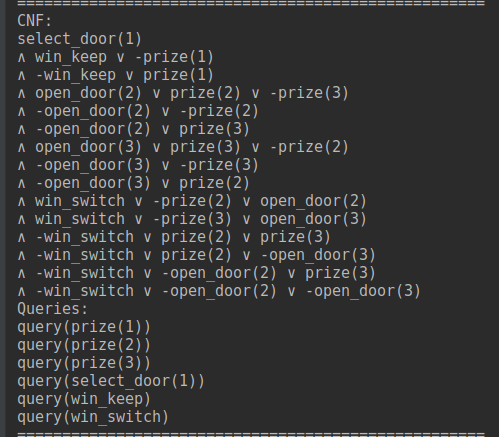
\includegraphics[width=7.5cm]{GroundProblogCNF.png}
  \label{CNF}
  \caption{Grounder problog cnf}
\end{figure}
TODO WEIGHTS

\section*{1.3}

\subsection*{1.3.1}
We will use mini2CD and Cachet as WMC counters.

\subsubsection*{mini2CD}

\begin{itemize}
	\item ENC1:
\begin{figure}[h!]
  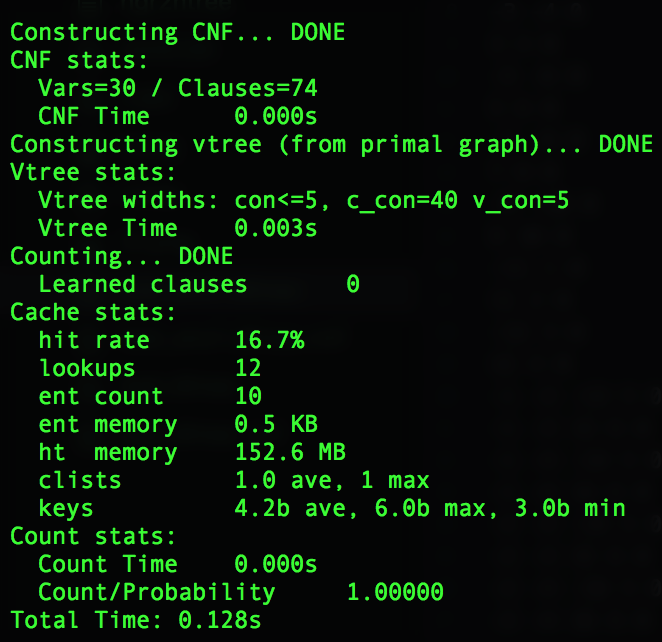
\includegraphics[width=7.5cm]{minic2d-ENC1.png}
  \label{CNF}
  \caption{Grounder problog cnf}
\end{figure}
	\item ENC2:
	\begin{figure}[h!]
  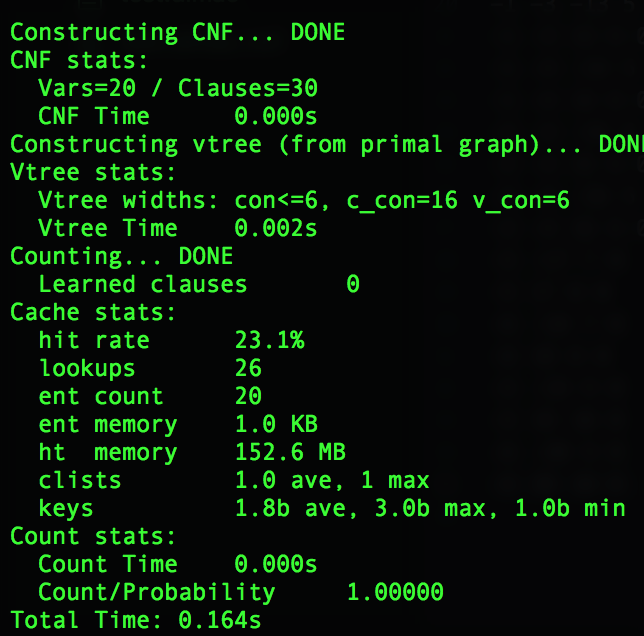
\includegraphics[width=7.5cm]{minic2d-ENC2.png}
  \label{CNF}
  \caption{Grounder problog cnf}
\end{figure}

	\item Prolog first:
\end{itemize}

\subsubsection*{Cachet}

\begin{itemize}
	\item ENC1:
	\item ENC2:
	\item Prolog first:
\end{itemize}


\subsection*{2. Difference between WMC's}
The three WMC we will compare are C2D, Cachet and SharpSAT.
%The differences between the different WMC's come from \cite{CHAVIRA2008772}.
%\subsubsection{Cachet vs jointree and recursive conditioning}
%Jointree and recursive conditioning only exploit topological structure thus they take no advantage of the massive determinism available in networks whilst Cachet does this.

\subsubsection*{C2D Vs Cachet}

The biggest difference between C2D and Cachet is that C2D keeps a track of the operation it has performed. This means that Cachet is not a compiler but C2D is. In \cite{CHAVIRA2008772} they note that Cachet could easily be transformed into a compiler. There are some other minor differences like they have a different way to implement decompositions but they also do variable splitting and caching in a different way.

%\subsubsection{ACE Vs Cachet}
%The biggest difference between them is that Cachet is a WMC by search and ACE is a WMC by compilation. In \cite{CHAVIRA2008772} they say that ACE and Cachet are almost equal in speed. They mention that they had to dissable some of ACE's built-in ways to optimze the search to make the comparisson fair. It can for example encode equal parameters, use structured resolutions, eclauses, ... \cite{CHAVIRA2008772} which optimize the search.
%They also differ in some other ways like the way they do decompositions, variable splitting and caching \cite{CHAVIRA2008772}.
%In \cite{CHAVIRA2008772} they note though that by enabling all the speed up features ACE has, that it is not always faster than Cachet. 

\subsubsection*{SharpSAT vs Cachet}
SharpSAT has an efficient way to cache components. This cache has a limited size and removes old entries using an utility function.
It also uses implicit boolean constraint propagation (BCP). This results in a smaller search space and reduces the cache size further.
SharpSAT also inherits different techniques from conventional SAT solvers. It inherits a clause learning and a fast BCP algorithm. It also has some things in common with Cachet: For selecting the branch variables, SharpSAT applies the VSADS algorithm from Cachet.
Cachet uses a string representation for components while SharpSAT uses a smart coding to store its components in a cache. \cite{SharpSAT}.

\subsubsection*{C2D vs SharpSAT}
The biggest difference between these two is that C2D is a compiler. A point they have in common is that they both use things from the literature. C2D creates a tree while SharpSAT doesn't.

\subsection*{3 Overview of computational requirements}
NOG DOEN.

\bibliography{biblio}
\bibliographystyle{plain}
\end{document}
